\documentclass{article}
\usepackage[italian]{babel}
\usepackage[tmargin=2cm,rmargin=1.5in,lmargin=1.5in,margin=0.85in,bmargin=2cm,footskip=.2in]{geometry}
\usepackage{siunitx}
\sisetup{separate-uncertainty=true, per-mode=fraction, parse-numbers=true}
\usepackage{caption}
\usepackage[T1]{fontenc}
\usepackage{bookmark}
\usepackage{mathcomp}
\usepackage{graphicx}
\usepackage{multicol}
\usepackage{booktabs}
\usepackage{amsmath,amsfonts,amsthm,amssymb,mathtools}
\hypersetup{
	pdftitle={Relazione pendolo fisico},
	colorlinks=true, linkcolor=doc!90,
	bookmarksnumbered=true,
	bookmarksopen=true
}
\usepackage{blindtext}
\usepackage{wrapfig}
\usepackage{listings}
\usepackage{xcolor}
\usepackage{float}
\usepackage{amsmath}
\usepackage{amssymb}
\usepackage{tikz}
\usepackage{titling}
\renewcommand\maketitlehooka{\null\mbox{}\vfill}
\renewcommand\maketitlehookd{\vfill\null}
\usepackage{multirow}
\usepackage{biblatex}
\definecolor{codegreen}{rgb}{0,0.6,0}
\definecolor{codegray}{rgb}{0.5,0.5,0.5}
\definecolor{codepurple}{rgb}{0.58,0,0.82}
\definecolor{backcolour}{rgb}{0.95,0.95,0.92}
\definecolor{doc}{rgb}{0,0,0}
\lstdefinestyle{code}{
    backgroundcolor=\color{backcolour},   
    commentstyle=\color{codegreen},
    keywordstyle=\color{magenta},
    numberstyle=\tiny\color{codegray},
    stringstyle=\color{codepurple},
    basicstyle=\ttfamily\footnotesize,
    breakatwhitespace=false,         
    breaklines=true,                 
    captionpos=b,                    
    keepspaces=true,                                     
    showspaces=false,                
    showstringspaces=false,
    showtabs=false,                  
    tabsize=2,
    inputencoding=ansinew,
    extendedchars=true,
    numbers=left,                    
    numbersep=5pt
}

\lstset{style=code}
\usepackage[varbb]{newpxmath}
\usepackage{circuitikz}
\captionsetup{labelfont={bf, sc}}
\title{Relazione pendolo fisico}
\author{Giosuè Aiello}
\date{\today}

\begin{document}
\begin{titlingpage}
    \begin{center}
        \vspace*{60pt} % Spazio dall'inizio della pagina

        {\Huge \textbf{\textsc{Relazione pendolo fisico}}} % Titolo in maiuscoletto
        \vspace{30pt} % Spazio dopo il titolo

        {\huge{Giosuè Aiello}} % Autore in corsivo e un po' più piccolo
        \vspace{20pt} % Spazio dopo l'autore

        {\large \today} % Data
    \end{center}
    
    \vfill % Riempie lo spazio verticale rimanente
\end{titlingpage}

\pagebreak

	\section{Scopo}
	Misurare il periodo di oscillazione di un pendolo fisico in funzione della distanza $d$ del punto $P$ in cui esso è vincolato e il centro di massa 
	\section{Premesse teoriche}

%-------------------------------------------------------------------------------------
\begin{figure}[h!]
	\centering
	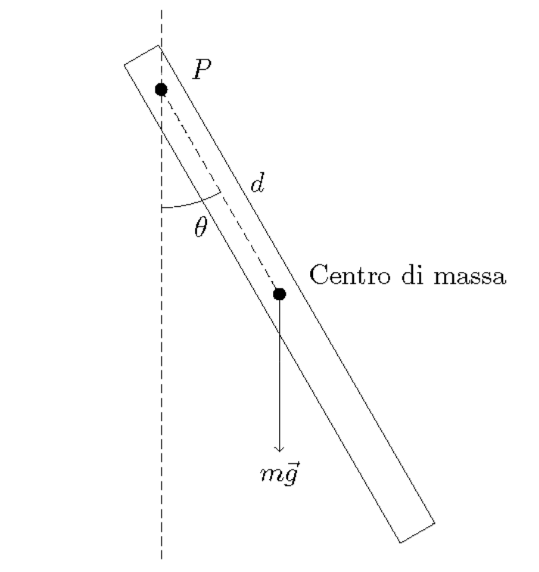
\includegraphics[scale=0.35]{pendolo_fisico.png}
	\caption{Schematizazzione del nostro apparato sperimentale}
	\label{fig:1}
\end{figure}
%-------------------------------------------------------------------------------------



\par\smallskip\noindent 	 Come mostrato in \textbf{Figura~\ref{fig:1}}, un corpo rigido fissato ad un punto di sospensione $P$ (che dista $d$ dal centro di massa) e soggetto alla gravità costituisce un pendolo fisico. Se viene spostato di un angolo $\theta$ dalla sua posizione di equilibrio, la gravità effettua un momento torcente sul centro di massa di questo corpo pari a
	$$
		\tau = -mgd\sin{\theta}
	$$
	e utilizzando la seconda equazione cardinale sappiamo che
	\begin{equation*}
		\tau = \frac{dL}{dt}
	\end{equation*}
	e sapendo che in questo caso il momento angolare è pari a $L = I\omega = I \frac{d\theta}{dt}$, abbiamo che
	\begin{equation*}
		\tau = \frac{dL}{dt} = I\ddot{\theta} = -mgd\sin{\theta}
	\end{equation*}
	dove $I$ rappresenta il momento di inerzia rispetto al punto P che, per il teorema di Hyugens-Steiner, risulta essere pari a:
	$$
		I = I_{CM} + md^2 = \frac{ml^2}{12} + md^2
	$$
	dove $m$ è la massa dell'asta, $l$ è la lunghezza complessiva dell'asta e $d$ è la distanza del punto $P$ dal centro di massa. \\
	Per angoli $\theta$ \emph{piccoli} (spiegherò alla fine di questa sezione che cosa si intende), possiamo utilizzare l'ipotesi delle piccole oscillazioni, per cui risulta che
	\begin{equation}
		\left( \frac{ml^2}{12} + md^2 \right) \ddot{\theta} = -mgd\theta \implies \ddot{\theta} = -\frac{gd}{\frac{l^2}{12} + d^2} \theta
	\end{equation}
	Come possiamo notare, quest'equazione differenziale è quella caratterizzante un moto armonico di pulsazione $\omega_0 = \sqrt{\frac{gd}{\frac{l^2}{12} + d^2}}$ dunque il periodo sarà di questo moto sarà banalmente
	\begin{equation}
		T = 2\pi * \sqrt{\frac{ \frac{l^2}{12} + d^2 }{gd}}
	\end{equation}
	Quindi si osserva che il periodo dipende dalla lunghezza dell'asta $l$ e dalla distanza $d$ del centro di massa dal punto di sospensione $P$, che sono due grandezze che ci dobbiamo accingere a misurare. \\
	Prima di procedere, specifichiamo che cosa voglia dire angoli \emph{piccoli}: il periodo, se non utilizziamo l'ipotesi delle piccole oscillazioni attorno al punto di equilibrio, si può dimostrare che essere ricondotto ad un integrale ellittico incompleto di prima specie di cui sappiamo calcolare l'espansione in serie di Taylor, che risulta essere pari a
	\begin{equation}
		T = 2 \pi \sqrt{\frac{\frac{l^2}{12} + d^2}{gd}} \left( 1 + \frac{\theta_0^2}{16} + o(\theta_0^2) \right)
	\end{equation}
	ora se risulta che
	 $$
\frac{T_0\theta^2_0}{16} \ll \sigma_T \quad \text{ovvero} \quad \frac{\theta^2_0}{16} \ll \frac{\sigma_T}{T_0} \quad \text{o, ancora} \quad \theta_0 \ll 4\sqrt{\frac{\sigma_T}{T_0}}
$$
allora possiamo trascurare i termini successivi all'ordine zero dello sviluppo in serie, dunque risulta che l'errore dipende esclusivamente dalla lunghezza $l$ dell'asta e dalla distanza $d$ del punto di sospensione dal centro di massa. 
\section{Strumenti e materiali}
	\textbf{Strumenti}:	
	\begin{itemize}
		\item Metro a nastro, con risoluzione pari a $0.1 \, \si{\centi\meter}$
		\item Cronometro con risoluzione pari a $0.01 \, \si{\second}$
	\end{itemize}
	\textbf{Materiali}:
	\begin{itemize}
		\item Asta metallica forata
		\item PC
		\item Supporto per la sospensione
	\end{itemize}

%----------------------------------------------------------------------------------------
\section{Descrizione delle misure}
Prima di procedere a misurare il periodo delle oscillazioni, ho misurato la lunghezza dell'asta $l$, che risulta essere pari a $l = (104.5 \pm 0.1) \, \si{\centi\meter}$. \\
Per stimare il centro di massa, siccome non posso supporre l'asta omogenea e questa presenta dei fori (quindi il centro di massa non si trova a metà del corpo), ho provato a mettere in equilibrio l'asta facendola sporgere dal banco di lavoro e vedere fin dove l'asta non cadeva. \\
Successivamente ho iniziato a misurare i periodi di oscillazioni in funzione della distanza $d$ del punto di sospensione dal centro di massa del corpo. Per ogni foro, che utilizzavo per tenere sospeso il pendolo, ho misurato $10$ periodi di oscillazione: infatti la maggiore fonte di errori in queste misurazioni deriva dal tempo di reazione con cui io vado a fermare il cronometro. \\

\pagebreak
%--------------------------------------------------------------------------------------------

\section{Analisi delle misure}
Come ho accennato nella descrizione delle misure, la misura sul tempo era dominata da errori accidentali dovuti al mio tempo di reazione nel fermare il cronometro. Dunque, ho considerato, come miglior stima del nostro misurando per ogni foro, la media aritmetica dei $10$ periodi di oscillazione che ho misurato e come incertezza ho utilizzato la deviazione standard della media. \\


\begin{wraptable}{r}{0.3\textwidth}
    \centering
    \begin{tabular}{c c} \toprule
        $T_i$ & $\sigma_i$ \\
        $[\si{\second}]$ & $[\si{\second}]$ \\ \toprule
        1.592 & 0.006 \\
        1.562 & 0.004 \\
        1.591 & 0.003 \\
        1.859 & 0.004 \\
        3.907 & 0.063 \\
        2.263 & 0.007 \\
        1.670 & 0.005 \\
        1.560 & 0.005 \\
        1.575 & 0.004 \\
        1.644 & 0.001 \\ \hline
    \end{tabular}
    \caption{Periodi con errore: in questa tabella sono espresse le misure del periodo di oscillazione al variare dalla distanza tra centro di massa e il punto di sospensione}
    \label{tab:1}
\end{wraptable}



\noindent Dunque il periodo di oscillazione del pendolo all'$i$-esimo foro risulta essere pari a
\begin{equation}
	T_i = \left( m_i \pm \sqrt{\frac{1}{10 \cdot 9}\sum_{j=1}^{10} (T_j - m_i)^2 } \right)
\end{equation}
dove con $m_i$ indico la media aritmetica dei periodi di oscillazione misurati all'$i$-esimo foro mentre con $T_j$ indico la $j$-esima misurazione compiuta a quel foro.Riporto qua accanto una tabella con i risultati delle misurazioni. \\\


\noindent Per un'analisi più accurata di questi dati, ho optato per il metodo del fit lineare, utilizzando il modello teorico del periodo nell'ipotesi delle piccole oscillazioni. Considerando, ad esempio il 5 foro con il periodo $T = 3.907 \pm 0.063$ s e l'errore relativo $\sigma_T/T_0 = 0.01613$, l'angolo limite risulta essere $\theta_0 \approx 29^\circ$. Poiché l'angolo limite è sufficientemente piccolo per tutti i fori, l'ipotesi delle piccole oscillazioni è giustificata. Pertanto, ho utilizzato il modello teorico del periodo $T = 2\pi\sqrt{l/g}$, con $l$ come parametro libero da stimare tramite il fit. Ciò è stato possibile utilizzando la funzione curve_fit della libreria scipy, confrontando la stima di $l$ effettuata dal fit con il valore reale noto.





\vspace{1.5cm}

\begin{figure}[H]
	\centering
	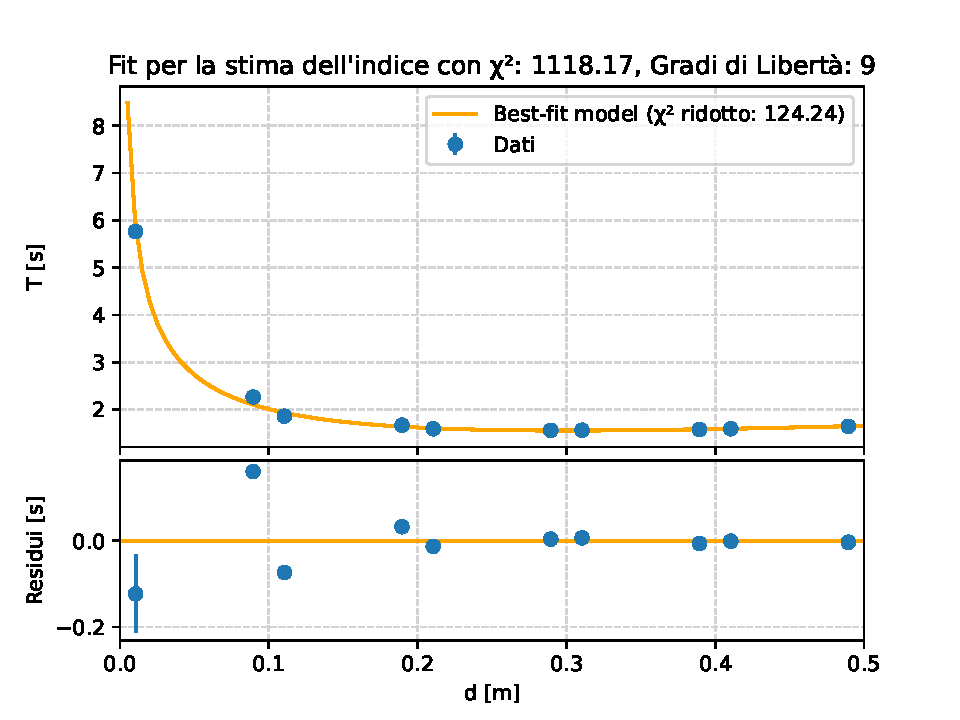
\includegraphics[scale=0.80]{Fit_e_residui.pdf}
	\caption{Grafico di \emph{best}-fit e residui: le incertezze sono presenti ma si vedono poco
	\label{fig:2}
	}
\end{figure}
\pagebreak
\begin{minipage}{1.0 \textwidth}
\noindent Prima di andare a commentare i grafici bisogra fare alcune considerazioni importanti, siccome in $d=0$ abbiamo un asintoto, gli errori sulle $d$ non sono trascurabili, dunque ho utilizzato il metodo degli errori efficaci. (che distano pochissime unita rispetto agli errori dei periodi precedentemente citati)\\\
\end{minipage}


\begin{minipage}{1.0 \textwidth}
I grafici nella \textbf{Figura~\ref{fig:2}} sono disposti dall'alto verso il basso, mostrando rispettivamente il grafico del fit e il grafico dei residui. Nel primo è rappresentata la relazione tra la distanza \( d \) [m] e il tempo \( T \) [s]. I punti blu rappresentano i dati sperimentali, mentre la curva arancione indica il modello di best-fit. Tale grafico sembra mostrare un buon accordo tra il nostro modello e i periodi, tuttavia non è così come vedremo tra poco.
\\\\
Il grafico dei residui mostra le differenze tra i dati sperimentali (punti in blu) e il modello di best-fit (in arancione). I residui sembrano essere vicini allo zero, mostrando un buon accordo tra modello e dati. Tuttavia, ingrandendo l'immagine, ci accorgiamo che la distanza tra il modello e tali punti è maggiore di molte barre di errore. Ciò non dovrebbe sorprendere, dato che puntando i vostri occhi sulla sommità della \textbf{Figura~\ref{fig:2}}, potrete osservare esposti il \( \chi^2 \) e i gradi di libertà, che immediatamente ci faranno notare una grande discrepanza tra i due.
\end{minipage}

\section{Conclusioni}
Considerando la notevole discrepanza tra il valore di $\chi^2$ e i gradi di libertà, il nostro modello teorico sembra discostarsi in modo significativo dai risultati empirici ottenuti nelle nostre misurazioni sperimentali. Ciononostante, l'andamento generale dei dati non è da trascurare, in quanto mostra una certa somiglianza con il modello. Il valore elevato di $\chi^2$ suggerisce la presenza di un consistente insieme di errori sistematici che avrebbero potuto influenzare in modo improprio il nostro risultato di $\chi^2$. Ad esempio, eventuali attriti non considerati nel modello, errori di misurazione o il metodo di cronometraggio manuale potrebbero aver introdotto scostamenti sistematici. 

Per cui un valore di $\chi^2$ elevato indica errori sistematici non considerati, ma non implica necessariamente che il modello teorico vada rigettato, infatti, l'andamento complessivo dei dati sembra seguire quello previsto dal modello, suggerendo che il modello colga gli aspetti essenziali del fenomeno osservato. \\\\In conclusione , non possiamo rigettare completamente il modello, ma dovremmo lavorare per identificare e correggere le possibili fonti di errore sistematico, in modo da ottenere un miglior accordo tra teoria e dati sperimentali.



\end{document}